% Created 2018-12-12 Wed 12:51
% Intended LaTeX compiler: pdflatex
\documentclass[11pt]{article}
\usepackage[utf8]{inputenc}
\usepackage[T1]{fontenc}
\usepackage{graphicx}
\usepackage{grffile}
\usepackage{longtable}
\usepackage{wrapfig}
\usepackage{rotating}
\usepackage[normalem]{ulem}
\usepackage{amsmath}
\usepackage{textcomp}
\usepackage{amssymb}
\usepackage{capt-of}
\usepackage{hyperref}
\usepackage{minted}
\usepackage[1.0in]{geometry}
\author{Mijeong Ban}
\date{\today}
\title{}
\hypersetup{
 pdfauthor={Mijeong Ban},
 pdftitle={},
 pdfkeywords={},
 pdfsubject={},
 pdfcreator={Emacs 26.1 (Org mode 9.1.9)}, 
 pdflang={English}}
\begin{document}


\section*{Part One. Statistical Report}
\label{sec:org68c24a5}

\section*{Part Two. Textbook Exercises}
\label{sec:orgf52f5d1}
\subsection*{11.42 Relationships among PCB congeners}
\label{sec:org47168dc}
Consider the following variables: PCB(the total amount of PCB) and four congeners: PCB52, PCB118, PCB138, and PCB180.
\subsubsection*{(a) Using numerical and graphical summaries, describe the distribution of each of these variables.}
\label{sec:org7d697bf}
\begin{table}[htbp]
\caption{Numerical Summaries}
\centering
\begin{tabular}{lrrrrrr}
Variable & Min & 1st Qu. & Median & Mean & 3rd Qu. & Max\\
\hline
PCB & 6.10 & 30.18 & 47.96 & 68.47 & 91.63 & 318.70\\
PCB52 & 0.020 & 0.228 & 0.477 & 0.958 & 0.892 & 9.060\\
PCB118 & 0.236 & 1.490 & 2.420 & 3.256 & 3.890 & 18.900\\
PCB138 & 0.640 & 3.180 & 4.920 & 6.827 & 8.650 & 32.300\\
PCB180 & 0.395 & 1.240 & 2.690 & 4.158 & 4.490 & 31.500\\
\end{tabular}
\end{table}

\begin{figure}[htbp]
\centering
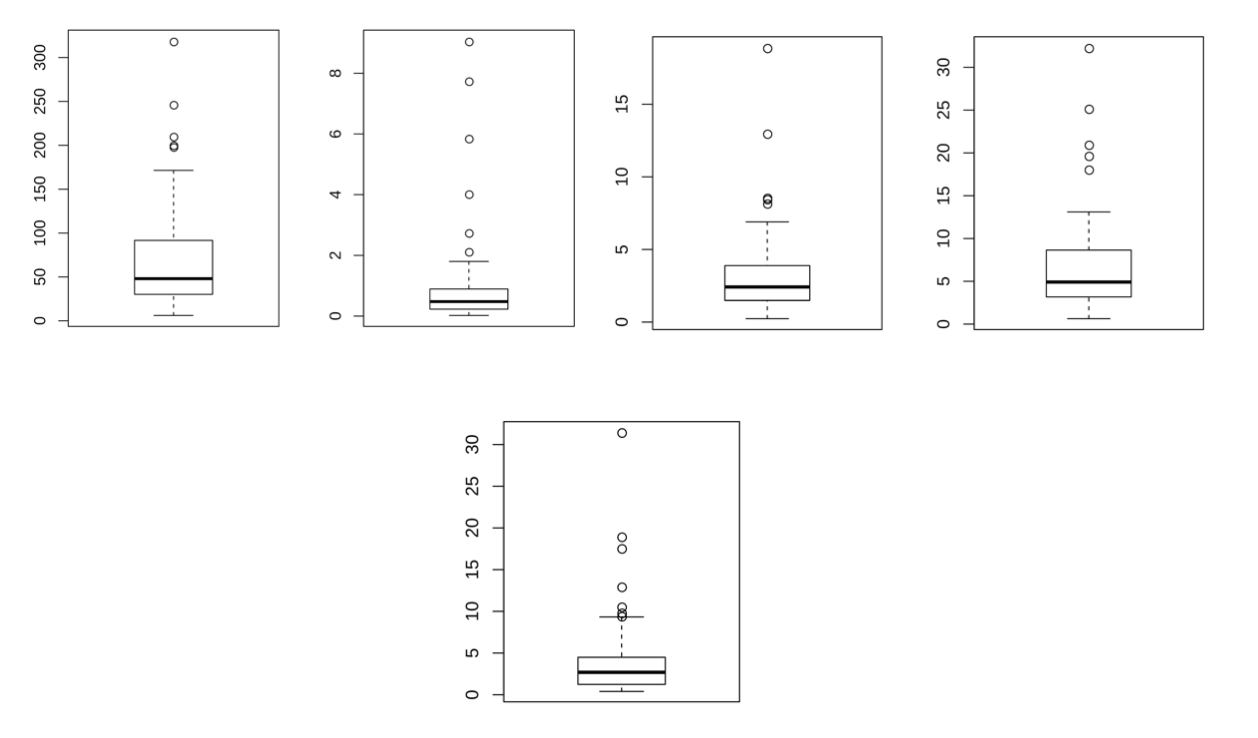
\includegraphics[width=.9\linewidth]{./graphs/image1.png}
\caption{Boxplots of PCB, PBC52, PCB118, PCB138 and PCB180}
\end{figure}
Figure 1 shows that the distribution of PCB and PCB180 is right skewed with about six outliers for both, while all the distribution of others are right skewed with about five outliers.  

\subsubsection*{(b) Using numerical and graphical summaries, describe the relationship between each pair of variables.}
\label{sec:org37a4074}
\begin{table}[htbp]
\caption{Correlations}
\centering
\begin{tabular}{llr}
Variable 1 & Variable 2 & Correlation\\
\hline
PCB & PCB52 & 0.5963572\\
PCB & PCB118 & 0.843298\\
PCB & PCB138 & 0.9288353\\
PCB & PCB180 & 0.8008549\\
PCB52 & PCB118 & 0.6849073\\
PCB52 & PCB138 & 0.3008983\\
PCB52 & PCB180 & 0.08692971\\
PCB118 & PCB138 & 0.7293792\\
PCB118 & PCB180 & 0.4374443\\
PCB138 & PCB180 & 0.8823022\\
\end{tabular}
\end{table}

\begin{center}
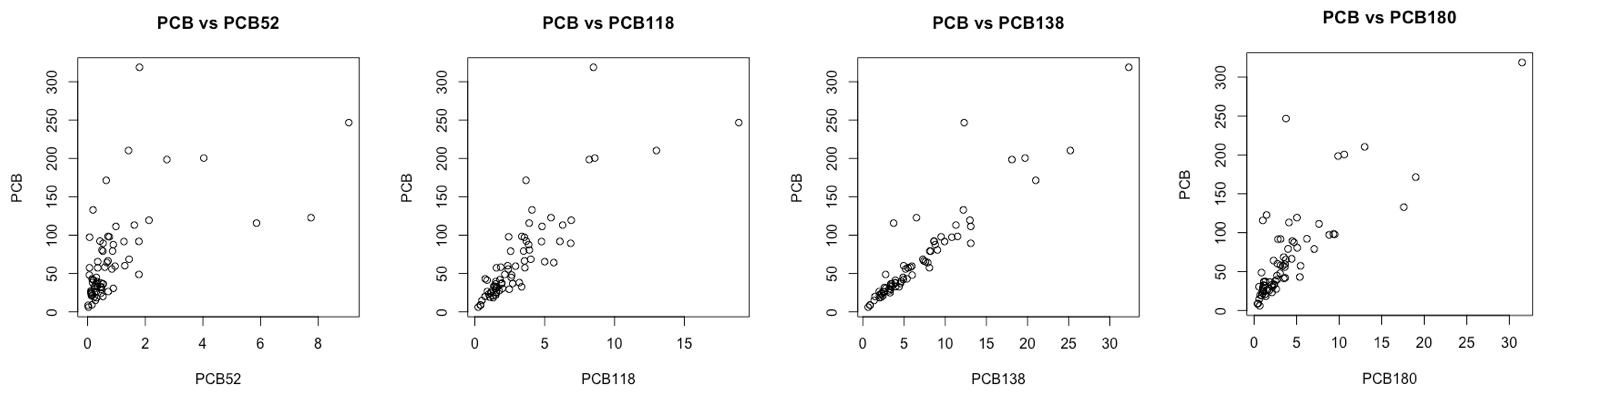
\includegraphics[width=.9\linewidth]{./graphs/image2.png}
\end{center}
\begin{center}
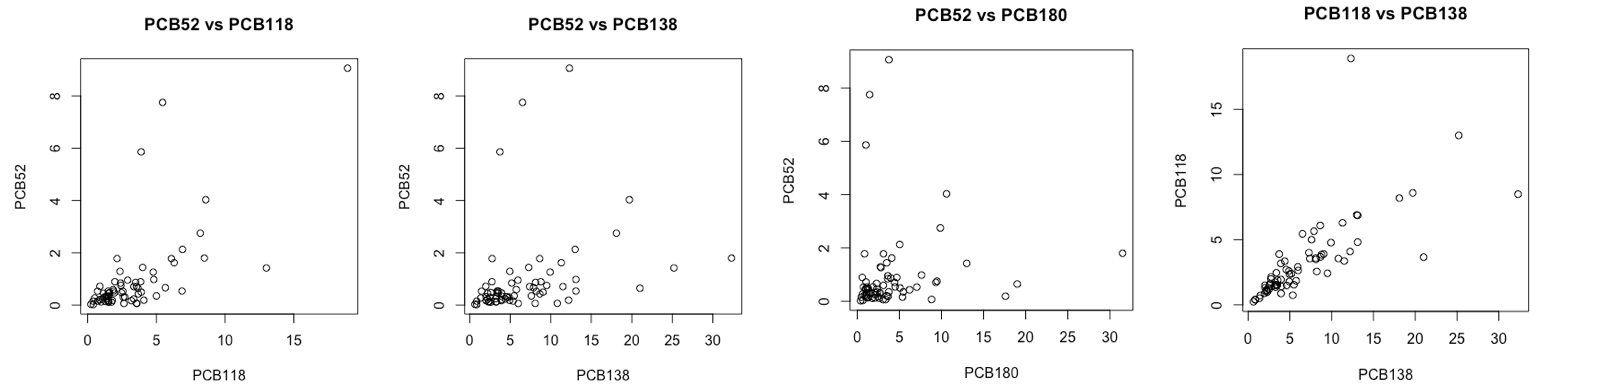
\includegraphics[width=.9\linewidth]{./graphs/image3.png}
\end{center}
\begin{center}
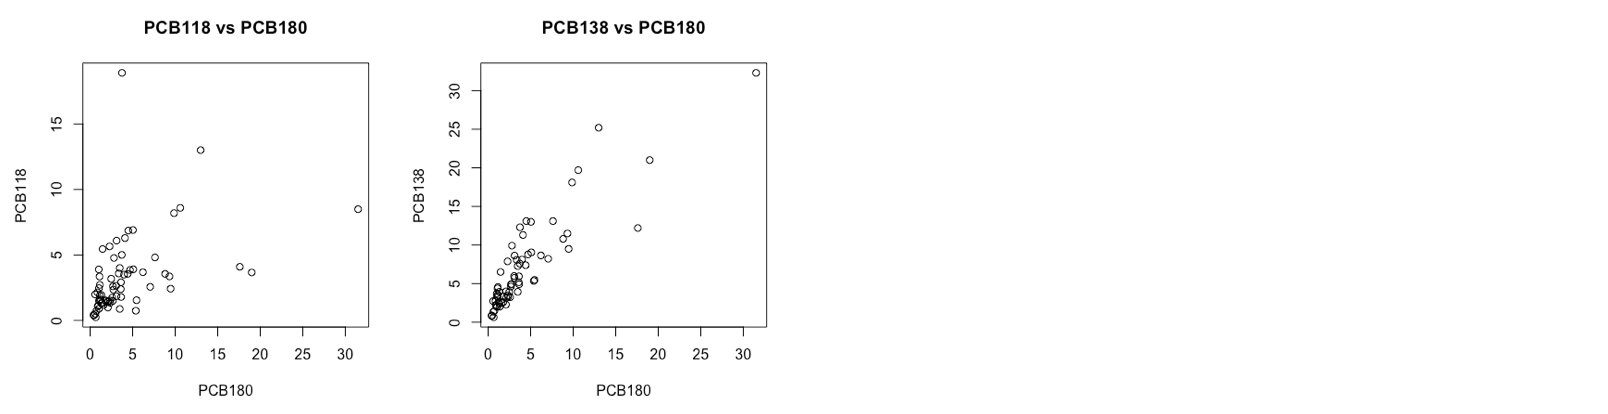
\includegraphics[width=.9\linewidth]{./graphs/image4.png}
\end{center}

\subsection*{11.43 Predictiong the total amount of PCB}
\label{sec:org8f389a6}
Use the four congeners PCB52, PCB118, PCB138, and PCB180 in a multiple regression to predict PCB. 
\subsubsection*{(a) Write the statistical model for this analysis. Include all assumptions.}
\label{sec:orgeabe84b}
The multiple linear regression model for the data with 69 observations:

y\(_{\text{i}}\) = \(\beta_{\text{0}}\) + \(\beta_{\text{1}}\)x\(_{\text{i1}}\) + \(\beta_{\text{2}}\)x\(_{\text{i2}}\) + \(\beta_{\text{3}}\)x\(_{\text{i3}}\) + \(\beta_{\text{4}}\)x\(_{\text{i4}}\) + i \emph{for} \emph{i = 1, 2, \ldots{} , 69}

We assume that the residuals are independent and are normally distributed. 
\subsubsection*{(b) Run the regression and summarize the results.}
\label{sec:org7038f75}
Multiple regression analyses were conducted to examine the relationship between PCB and four congeners. Running the multiple regression model in R with the four congeners produced the following:
\begin{verbatim}

subdf <- subset(df, select = c("pcb", "pcb52", "pcb118", "pcb138", "pcb180"))
> lm1 = lm(pcb~pcb52 + pcb118 + pcb138 + pcb180, data=subdf)
> coef(lm1)
(Intercept)       pcb52      pcb118      pcb138      pcb180 
  0.9369203  11.8726953   3.7610694   3.8842264   4.1823010 
> summary(lm1)

Call:
lm(formula = pcb ~ pcb52 + pcb118 + pcb138 + pcb180, data = subdf)

Residuals:
     Min       1Q   Median       3Q      Max 
-22.0864  -2.4554   0.0278   2.7726  22.5487 

Coefficients:
            Estimate Std. Error t value Pr(>|t|)    
(Intercept)   0.9369     1.2293   0.762    0.449    
pcb52        11.8727     0.7290  16.287  < 2e-16 ***
pcb118        3.7611     0.6424   5.855 1.79e-07 ***
pcb138        3.8842     0.4978   7.803 7.19e-11 ***
pcb180        4.1823     0.4318   9.687 3.64e-14 ***
---
Signif. codes:  0 ‘***’ 0.001 ‘**’ 0.01 ‘*’ 0.05 ‘.’ 0.1 ‘ ’ 1

Residual standard error: 6.382 on 64 degrees of freedom
Multiple R-squared:  0.9891,	Adjusted R-squared:  0.9885 
F-statistic:  1456 on 4 and 64 DF,  p-value: < 2.2e-16

> anova(lm1)
Analysis of Variance Table

Response: pcb
          Df Sum Sq Mean Sq  F value    Pr(>F)    
pcb52      1  85302   85302 2094.273 < 2.2e-16 ***
pcb118     1  85429   85429 2097.405 < 2.2e-16 ***
pcb138     1  62693   62693 1539.202 < 2.2e-16 ***
pcb180     1   3822    3822   93.834  3.64e-14 ***
Residuals 64   2607      41                       
---
Signif. codes:  0 ‘***’ 0.001 ‘**’ 0.01 ‘*’ 0.05 ‘.’ 0.1 ‘ ’ 1
\end{verbatim}
\begin{itemize}
\item We gathered the following from the results of the regression:
\label{sec:org0104edf}
\begin{itemize}
\item The multiple R\(^{\text{2}}\) = 0.989
\item The residual SE = 6.249
\end{itemize}
\end{itemize}

\item Test 1
\label{sec:org0fe9b4b}

H\(_{\text{0}}\) : \(\beta_{\text{0}}\) = \(\beta_{\text{1}}\) = \(\beta_{\text{2}}\) = \(\beta_{\text{3}}\) = \(\beta_{\text{4}}\) = 0

H\(_{\text{1}}\) : \(\beta_{\text{0}}\) \(\neq\) 0 \(\vee\) \(\beta_{\text{1}}\) \(\neq\) 0 \(\vee\) \(\beta_{\text{2}}\) \(\neq\) 0 \(\vee\) \(\beta_{\text{3}}\) \(\neq\) 0 \(\vee\) \(\beta_{\text{4}}\) \(\neq\) 0

Since there is at least one \(\beta_{\text{n}}\) \(\neq\) 0, we reject H\(_{\text{0}}\) 

\item Test 2
\label{sec:orgb751dd8}

H\(_{\text{0}}\) = \(\beta_{\text{j}}\) = 0, \emph{j = 0, 1, 2, 3}

H\(_{\text{1}}\) = \(\beta_{\text{j}}\) \(\neq\) 0

All regression coefficients are significantly different from 0 with the except of 0.94. We found that R\(^{\text{2}}\) = 0.989, meaning that 98.9\% of variation in PCB is from PCB52, PCB118, PCB138 and PCB180.
\end{itemize}

\subsubsection*{(c) Examine the residuals. Do they appear to be approximately Normal? When you plot them versus each of the explanatory variables, are any patterns evident?}
\label{sec:org9ff1117}
\begin{center}
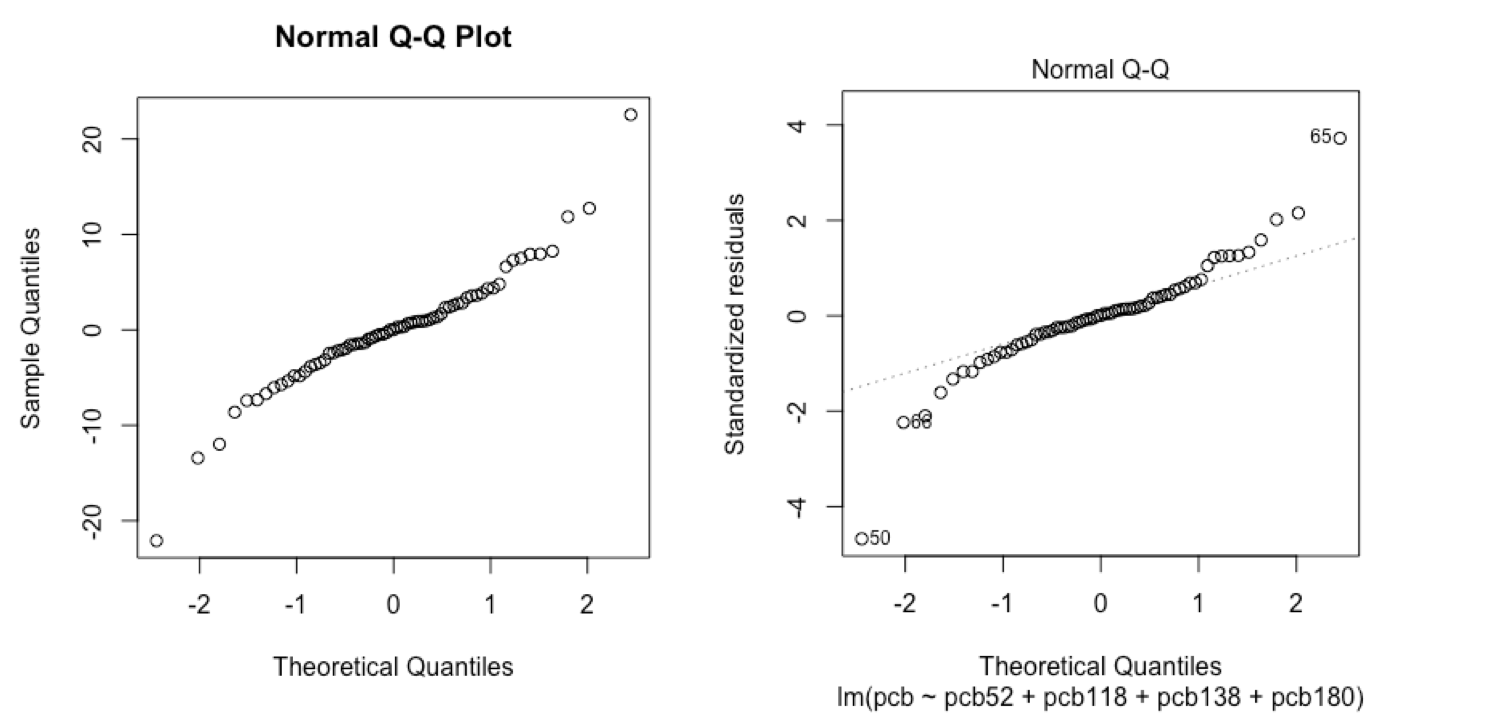
\includegraphics[width=.9\linewidth]{./graphs/image5.png}
\end{center}
According to the graphs, the residuals shows two clear outliers and shows that the residuals are approximately normal. Rhere are no other patterns in the explanatory variables of note. 

\subsection*{11.44 Adjusting the analysis for potential outliers.}
\label{sec:org9ae6c75}
The examination of the residuals in part (c) of the previous exercise suggests that there may be two outliers, one with a high residual and one with a low residual. 
\subsubsection*{(a) Because of safety issues, we are more concerned about underestimating PCB in a specimen than about overestimating. Give the specimen number for each of the two suspected outliers. Which one corresponds to an overestimate of PCB?}
\label{sec:org15f5465}
\begin{center}
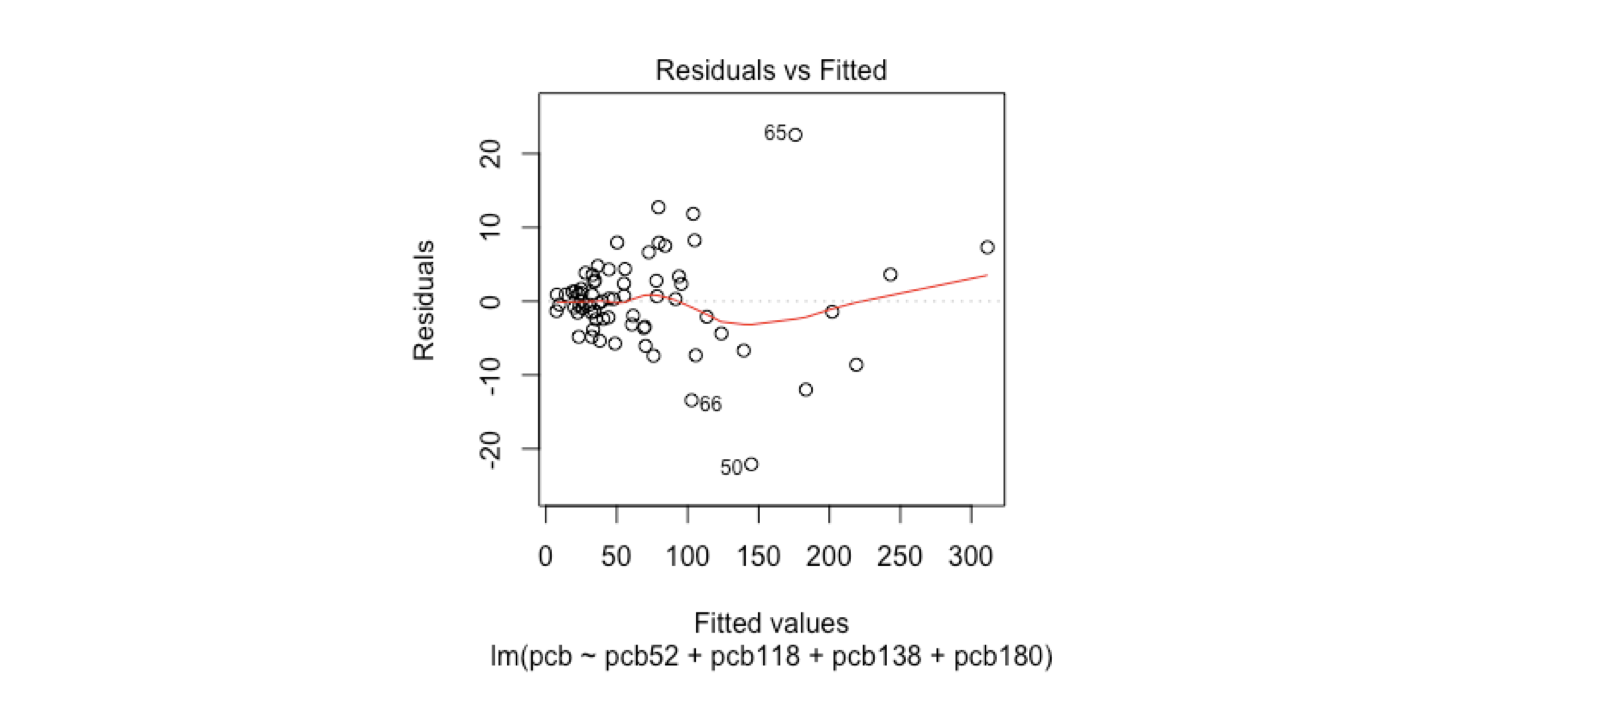
\includegraphics[width=.9\linewidth]{./graphs/image6.png}
\end{center}
The specimen 50 and 65 are the two data points that are outliers. Specimen 65 corresponds to an overestimate of PCB due to its higher residual value. 

\subsubsection*{(b) Rerun the analysis with the two suspected outliers deleted, summarize these results, and compare them with those you obtained in the previous exercise.}
\label{sec:orgee4473a}

\begin{verbatim}
(Intercept)       pcb52      pcb118      pcb138      pcb180 
   1.627718   14.442021    2.599636    4.054061    4.108575 
> summary(lm2)
Call:
lm(formula = pcb ~ pcb52 + pcb118 + pcb138 + pcb180, data = subdf2)

Residuals:
     Min       1Q   Median       3Q      Max 
-12.2421  -2.1762  -0.1378   1.7036  14.2051 

Coefficients:
            Estimate Std. Error t value Pr(>|t|)    
(Intercept)   1.6277     0.8858   1.838   0.0709 .  
pcb52        14.4420     0.6960  20.751  < 2e-16 ***
pcb118        2.5996     0.5164   5.034 4.40e-06 ***
pcb138        4.0541     0.3752  10.805 6.89e-16 ***
pcb180        4.1086     0.3175  12.942  < 2e-16 ***
---
Signif. codes:  0 ‘***’ 0.001 ‘**’ 0.01 ‘*’ 0.05 ‘.’ 0.1 ‘ ’ 1

Residual standard error: 4.555 on 62 degrees of freedom
Multiple R-squared:  0.9941,	Adjusted R-squared:  0.9938 
F-statistic:  2629 on 4 and 62 DF,  p-value: < 2.2e-16

> anova(lm2)
Analysis of Variance Table
Response: pcb
          Df Sum Sq Mean Sq F value    Pr(>F)    
pcb52      1  84307   84307  4062.7 < 2.2e-16 ***
pcb118     1  68740   68740  3312.6 < 2.2e-16 ***
pcb138     1  61670   61670  2971.9 < 2.2e-16 ***
pcb180     1   3476    3476   167.5 < 2.2e-16 ***
Residuals 62   1287      21                      
---
Signif. codes:  0 ‘***’ 0.001 ‘**’ 0.01 ‘*’ 0.05 ‘.’ 0.1 ‘ ’ 1
\end{verbatim}
The residual standard error has been decreased without the suspected outliers, from 6.382 to 4.555. R\(^{\text{2}}\) has also increased from 0.989 to 0.994, meaning the predictions with this dataset become more accurate. 

\subsection*{11.45 More on predicting the total amount of PCB.}
\label{sec:org5fe0523}
Run a regression to predict PCB using the variables PCB52, PCB118, and PCB138. Note that this is similar to the analysis that you did in Exercise 11.43, with the change that PCB 180 is not included as an explanatory variable. 
\subsubsection*{(a) Summarize the results.}
\label{sec:org7835577}

\begin{verbatim}
> coef(lm3)
(Intercept)       pcb52      pcb118      pcb138 
 -1.0183987  12.6441934   0.3131051   8.2545867 
> summary(lm3)
Call:
lm(formula = pcb ~ pcb52 + pcb118 + pcb138, data = subdf3)

Residuals:
     Min       1Q   Median       3Q      Max 
-29.6219  -3.3502   0.8791   3.3785  29.5217 

Coefficients:
            Estimate Std. Error t value Pr(>|t|)    
(Intercept)  -1.0184     1.8895  -0.539    0.592    
pcb52        12.6442     1.1291  11.198   <2e-16 ***
pcb118        0.3131     0.8333   0.376    0.708    
pcb138        8.2546     0.3279  25.177   <2e-16 ***
---
Signif. codes:  0 ‘***’ 0.001 ‘**’ 0.01 ‘*’ 0.05 ‘.’ 0.1 ‘ ’ 1

Residual standard error: 9.945 on 65 degrees of freedom
Multiple R-squared:  0.9732,	Adjusted R-squared:  0.972 
F-statistic: 786.7 on 3 and 65 DF,  p-value: < 2.2e-16

> anova(lm3)
Analysis of Variance Table
Response: pcb
          Df Sum Sq Mean Sq F value    Pr(>F)    
pcb52      1  85302   85302  862.48 < 2.2e-16 ***
pcb118     1  85429   85429  863.77 < 2.2e-16 ***
pcb138     1  62693   62693  633.88 < 2.2e-16 ***
Residuals 65   6429      99                      
---
Signif. codes:  0 ‘***’ 0.001 ‘**’ 0.01 ‘*’ 0.05 ‘.’ 0.1 ‘ ’ 1
\end{verbatim}
We can get the following values from the results of the regression:
\begin{itemize}
\item The squared multiple correlation coeffiicient R\(^{\text{2}}\) = 0.973
\item The residual standard error SE = 9.942
\end{itemize}

\subsubsection*{(b) In this analysis, the regression coefficient for PCB118 is not statistically significant. Give the estimate of the coefficient and the associated \emph{P}-value.}
\label{sec:org8dab337}

\begin{itemize}
\item Using a significance level \(\alpha\) = 0.05, Specimen PCB118 has a regression coefficient = 0.313 and \emph{P}-value = 0.708
\item Significance Test: 0.708 > 0.05 (Reject when P > \(\alpha\))
\item \emph{P}-value is much larger than the significance level. Therefore, we reject the null hypothesis.
\end{itemize}

\subsubsection*{(c) Find the estimate of the coefficient for PCB118 and the associated \emph{P}-value for the model analyzed the Ecercise 11.43.}
\label{sec:orgc521627}
\begin{itemize}
\item Using a significance level \(\alpha\) = 0.05, Specimen PCB118(from Exercise 11.43) has a regression coefficient = 3.7611 and \emph{P}-value = 0.000
\item Significance Test: 0.000 < 0.05 (Reject when P > \(\alpha\))
\item \emph{P}-value is much smaller than the significance level. Therefore, we don't reject the null hypothesis.
\end{itemize}

\subsubsection*{(d) Using the results in parts (b) and (c), write a short paragraph explaining how the inclusion of other variables in a multiple regression can have an effect on the estimate of a particular coefficient and the results of the associated significance test.}
\label{sec:org7914596}
As parts (b) and (c) of this exercise show, the statistical significance of another variable is changed entirely, just by removing one explanatory variable. In the case above, removing the explanatory variable PCB180 made another explanatory variable PCB118 no longer statistically significant, along with drastically changing the variables corresponding regression coefficient and P-value. 

\subsection*{11.46 Multiple regression model for total TEQ}
\label{sec:org521c6e2}
\subsubsection*{(a) Consider using a multiple regression to predict TEQ using the tree components TEQPCB, TEQDIOXIN, and TEQFURAN as explanatory variables. Write the multiple regression model in the form: TEQ = \(\beta_{\text{0}}\) + \(\beta_{\text{1}}\)TEQPCB + \(\beta_{\text{2}}\)TEQDIOXIN + \(\beta_{\text{3}}\)TEQFURAN + \(\epsilon\). Give numerical values for the parameters \(\beta_{\text{0}}\), \(\beta_{\text{1}}\), \(\beta_{\text{2}}\), and \(\beta_{\text{3}}\).}
\label{sec:org8f84d30}

\(\beta_{\text{0}}\) = 0, \(\beta_{\text{1}}\) = 1, \(\beta_{\text{2}}\) = 1, \(\beta_{\text{3}}\) = 1

TEQ = 0 + 1 * TEQPCB + 1 * TEQDIOXIN + 1 * TEQFURAN

\subsubsection*{(b) The multiple regression model assumes that the \(\epsilon\)'s are Normal with mean zero and standard deviation \(\sigma\). What is the numerical value of \(\sigma\)?}
\label{sec:org32de0e7}
\(\sigma\) = s = 7.95e-6
\subsubsection*{(c) Use software to run this regression and summarize the results.}
\label{sec:orgc07bb49}

\begin{verbatim}
> lm4 <- lm(teq~teqpcb+teqdioxin+teqfuran, data=df)
> coef(lm4)
 (Intercept)       teqpcb    teqdioxin     teqfuran 
3.425522e-07 1.000001e+00 1.000000e+00 1.000001e+00 
> summary(lm4)

Call:
lm(formula = teq ~ teqpcb + teqdioxin + teqfuran, data = df)

Residuals:
       Min         1Q     Median         3Q        Max 
-5.638e-06 -2.844e-06 -1.680e-06 -1.130e-06  3.714e-05 

Coefficients:
             Estimate Std. Error   t value Pr(>|t|)    
(Intercept) 3.426e-07  1.917e-06 1.790e-01    0.859    
teqpcb      1.000e+00  8.239e-07 1.214e+06   <2e-16 ***
teqdioxin   1.000e+00  1.761e-06 5.677e+05   <2e-16 ***
teqfuran    1.000e+00  5.664e-06 1.766e+05   <2e-16 ***
---
Signif. codes:  0 ‘***’ 0.001 ‘**’ 0.01 ‘*’ 0.05 ‘.’ 0.1 ‘ ’ 1

Residual standard error: 7.95e-06 on 65 degrees of freedom
Multiple R-squared:      1,	Adjusted R-squared:      1 
F-statistic: 9.581e+11 on 3 and 65 DF,  p-value: < 2.2e-16

> anova(lm4)
Analysis of Variance Table
Response: teq
          Df  Sum Sq Mean Sq    F value    Pr(>F)    
teqpcb     1 152.801 152.801 2.4174e+12 < 2.2e-16 ***
teqdioxin  1  26.903  26.903 4.2562e+11 < 2.2e-16 ***
teqfuran   1   1.970   1.970 3.1174e+10 < 2.2e-16 ***
Residuals 65   0.000   0.000                         
---
Signif. codes:  0 ‘***’ 0.001 ‘**’ 0.01 ‘*’ 0.05 ‘.’ 0.1 ‘ ’ 1
\end{verbatim}
\begin{itemize}
\item We gathered the following values from the results of the regression:
\label{sec:org92f6604}
\begin{itemize}
\item Multiple R-squared R\(^{\text{2}}\) = 1
\item Residual standard error SE = 7.95e-06 \(\approx\) 0
\end{itemize}
\end{itemize}

\item Test 1
\label{sec:org92b12e5}

H\(_{\text{0}}\) : \(\beta_{\text{0}}\) = \(\beta_{\text{1}}\) = \(\beta_{\text{2}}\) = \(\beta_{\text{3}}\) = \(\beta_{\text{4}}\) = 0

H\(_{\text{1}}\) : \(\beta_{\text{0}}\) \(\neq\) 0 \(\vee\) \(\beta_{\text{1}}\) \(\neq\) 0 \(\vee\) \(\beta_{\text{2}}\) \(\neq\) 0 \(\vee\) \(\beta_{\text{3}}\) \(\neq\) 0 \(\vee\) \(\beta_{\text{4}}\) \(\neq\) 0

Since there is at least one \(\beta_{\text{n}}\) \(\neq\) 0, we reject H\(_{\text{0}}\)

\item Test 2
\label{sec:org063476a}

H\(_{\text{0}}\) = \(\beta_{\text{j}}\) = 0, \emph{j = 0, 1, 2, 3}

H\(_{\text{1}}\) = \(\beta_{\text{j}}\) \(\neq\) 0

All regression coefficients are significantly different from 0 with the exception of the constant R\(^{\text{1}}\) = 1, meaning 100\% of TEQ is explained by TEQPCB, TEQDIOXIN and TEQFURAN.
\end{itemize}

\subsection*{11.47 Multiple regression model for total TEQ, cont.}
\label{sec:org145fa4a}
\begin{verbatim}
Call:
lm(formula = teq ~ pcb52 + pcb118 + pcb138 + pcb180, data = df)

Residuals:
    Min      1Q  Median      3Q     Max 
-1.6655 -0.6000 -0.1814  0.5162  2.7025 

Coefficients:
             Estimate Std. Error t value Pr(>|t|)    
(Intercept)  1.059965   0.184450   5.747 2.73e-07 ***
pcb52       -0.097277   0.109383  -0.889  0.37716    
pcb118       0.306184   0.096388   3.177  0.00229 ** 
pcb138       0.105786   0.074697   1.416  0.16156    
pcb180      -0.003905   0.064784  -0.060  0.95212    
---
Signif. codes:  0 ‘***’ 0.001 ‘**’ 0.01 ‘*’ 0.05 ‘.’ 0.1 ‘ ’ 1

Residual standard error: 0.9576 on 64 degrees of freedom
Multiple R-squared:  0.6769,	Adjusted R-squared:  0.6568 
F-statistic: 33.53 on 4 and 64 DF,  p-value: 4.489e-15

> summary(aov(lm5))
            Df Sum Sq Mean Sq F value   Pr(>F)    
pcb52        1  29.85   29.85  32.553 3.21e-07 ***
pcb118       1  83.61   83.61  91.174 6.30e-14 ***
pcb138       1   9.52    9.52  10.378  0.00201 ** 
pcb180       1   0.00    0.00   0.004  0.95212    
Residuals   64  58.69    0.92                     
---
Signif. codes:  0 ‘***’ 0.001 ‘**’ 0.01 ‘*’ 0.05 ‘.’ 0.1 ‘ ’ 1
\end{verbatim}
\subsubsection*{The regression equation used:}
\label{sec:org95b6a93}
TEQ = 1.06 − 0.097 ∗ PCB52 + 0.306 ∗ PCB118 + 0.106 ∗ PCB138 − 0.0039 ∗ PCB180
\begin{itemize}
\item Multiple R-squared R\(^{\text{2}}\) = 0.6772
\item Residual standard error SE = 0.9571
\end{itemize}

\subsubsection*{Significance Test:}
\label{sec:org070d237}
\begin{itemize}
\item H\(_{\text{0}}\) = \(\beta_{\text{1}}\) = \(\beta_{\text{2}}\) = \(\beta_{\text{3}}\) = \(\beta_{\text{4}}\) = 0
\item H\(_{\text{a}}\) : one or more \(\beta\) \(\neq\) 0
\item The \emph{P}-value of both PCB118 and constant are close to 0, but still significantly different, therefore we reject null hypothesis.
\end{itemize}

\begin{center}
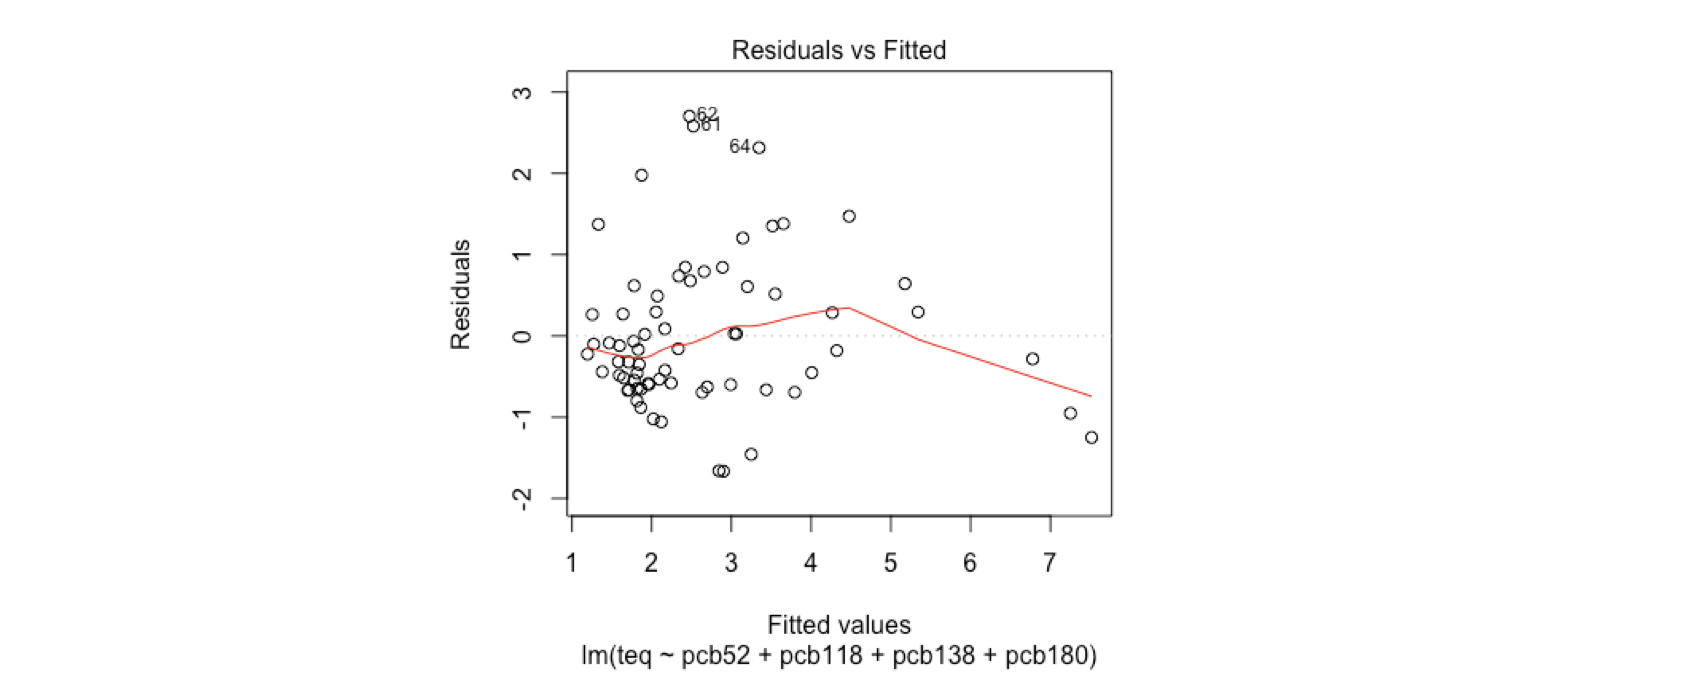
\includegraphics[width=.9\linewidth]{./graphs/image7.png}
\end{center}
When plotting the residuals, the data is skewed right but does not include any other obvious patterns. 
\end{document}
